\chapter{Ralentissements des neutrons}
\section{Introduction}
La diminution de l'énergie des neutrons de $E_{fission}$ à $E_{th}$ peut se faire par scattering 
élastique ou inélastique. Regardons les deux cas
\begin{enumerate}
\item \textit{Collisions inélastiques} :: l faut que l'énergie du neutron incident soit supérieur au 
premier niveau d'excitation du noyau. Celui ci vaut
\begin{itemize}
\item[$\bullet$] 1 MeV pour les noyaux légers
\item[$\bullet$] 0.1 MeV pour les noyaux lourds
\end{itemize}
Les collisions inélastiques avec des noyaux lourds sont possibles, mais pour des valeurs d'énergie
bien supérieures au domaine de résonance.
\item \textit{Collisions élastiques} : celle-ci n'est pas efficace avec les noyaux lourds et il faut
dès lors utiliser des noyaux légers, qui joueront le rôle de \textit{modérateurs}.
\end{enumerate}

\section{Ralentissement via scattering inélastique}
\subsection{Cinématique}
	\begin{wrapfigure}[11]{l}{10cm}
	\vspace{-5mm}
	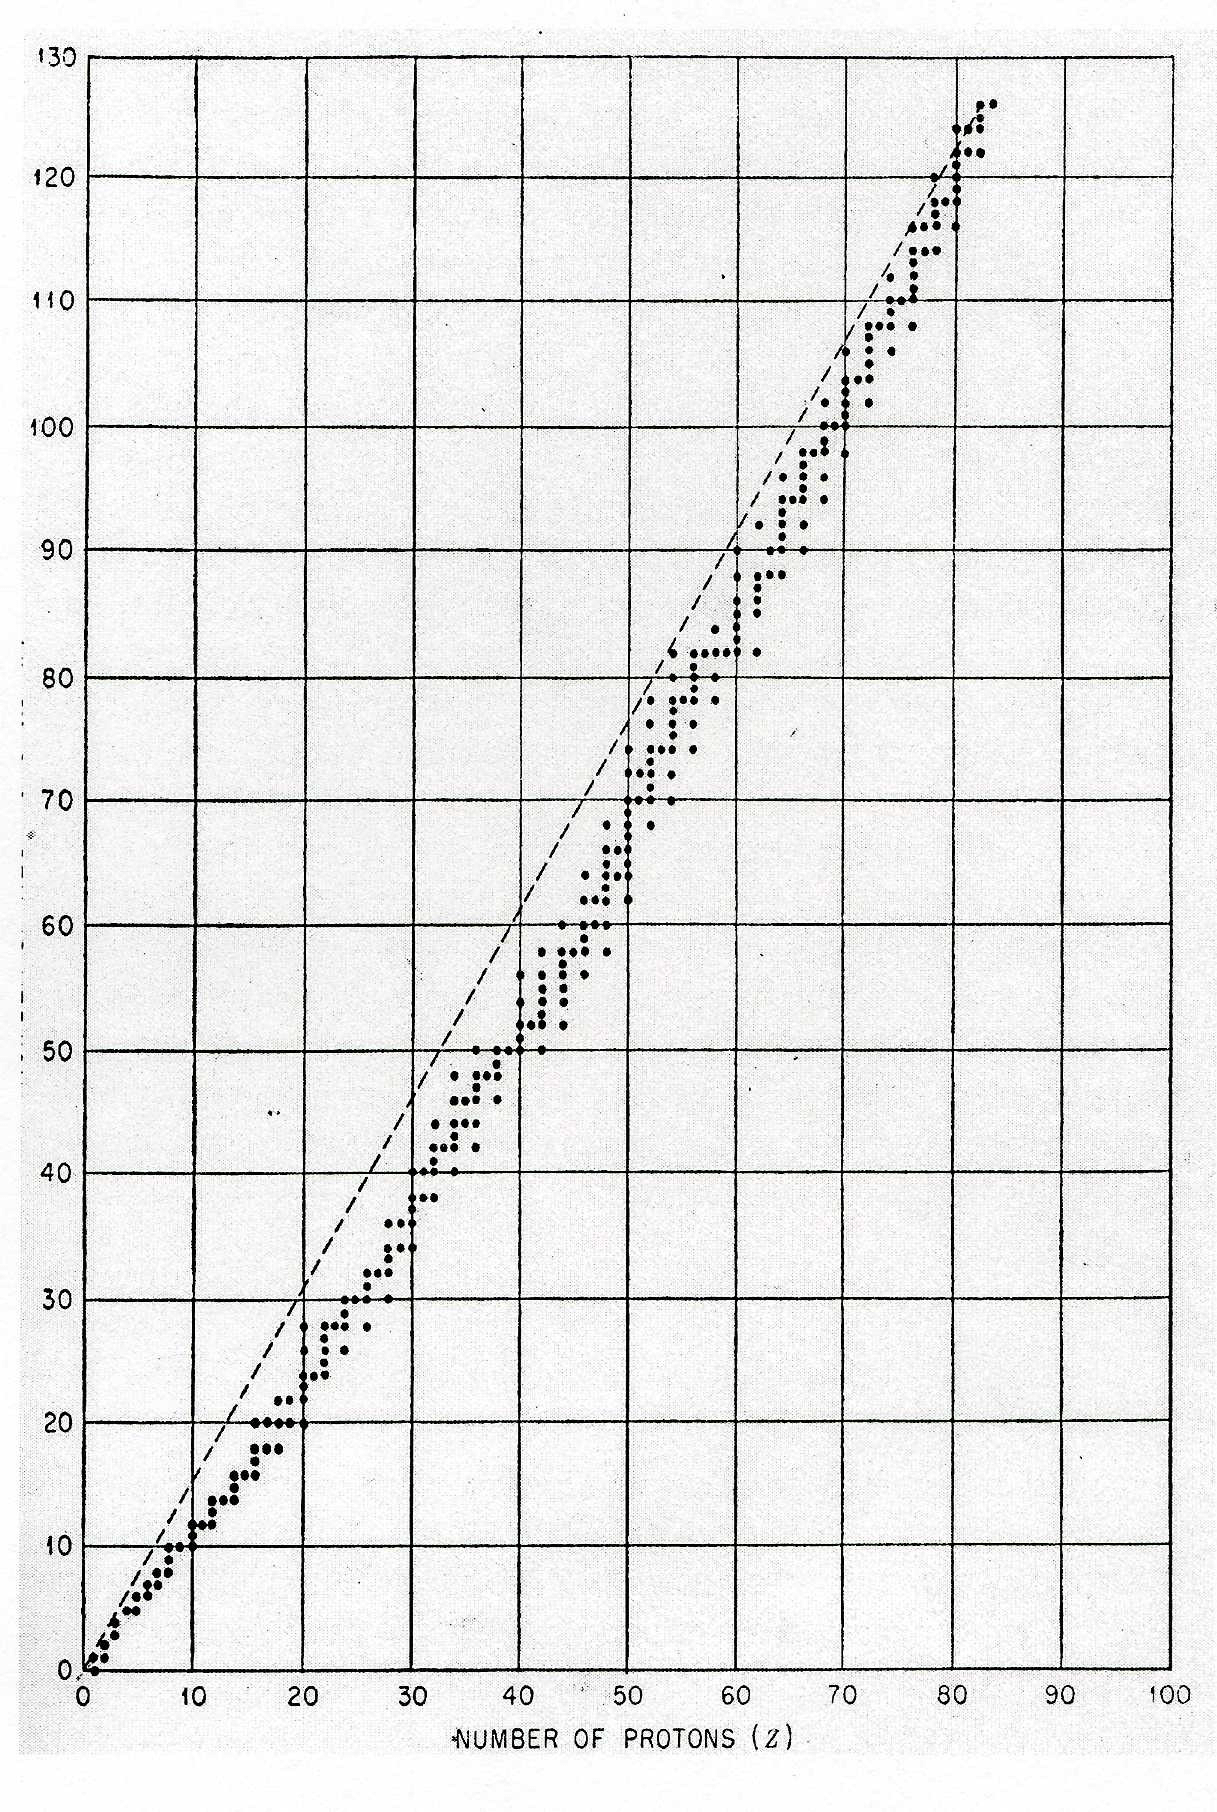
\includegraphics[scale=0.4]{ch7/image1.png}
	\captionof{figure}{ }
	\end{wrapfigure}
	Le but est d'étudier l'effet des collisions élastiques sur le ralentissement. Dans le système de 
	coordonnées \textit{absolue}, le neutron est initialement caractérisé par $\bar v'$ et $E'$ avant 
	collision et après par $\bar v$ et $E$. Dans le système du \textit{centre de masse}, il faut 
	considérer une vitesse relative avant la collision\footnote{$A$ est la masse du noyau et 1 la
	masse du neutron, on comprend alors le sens du dénominateur servant à la pondération.}. Par 
	collision élastique, la vitesse relative possède une amplitude similaire à la situation avant 
	collision mais une direction modifiée. \\
	
	La vitesse du centre de masse et celle du neutron sont donc conservée dans le mouvement relatif
	mais il y a modification de la direction.\\
	
	La vitesse, étant relative, est donnée par la somme de la vitesse du centre de masse $\bar v_G$ et 
	la vitesse relative $\bar v_r$
	\begin{equation}
	\bar v = {\bar v_G} + {\bar v_r} = \frac{{v'}}{{A + 1}}(\bar \Omega ' + A{\bar \Omega _r})
	\end{equation}
	En prenant les modules carré de part et d'autre et que l'on effectue le ratio de l'énergie 
	finale sur l'énergie incidente, on trouve
	\begin{equation}
	\frac{E}{{E'}} = \frac{{{v^2}}}{{v{'^2}}} = \frac{{{A^2} + 2A{\mu _r} + 1}}{{{{(A + 1)}^2}}}
	\end{equation}
	
	\begin{wrapfigure}[7]{r}{2.5cm}
	\vspace{-5mm}
	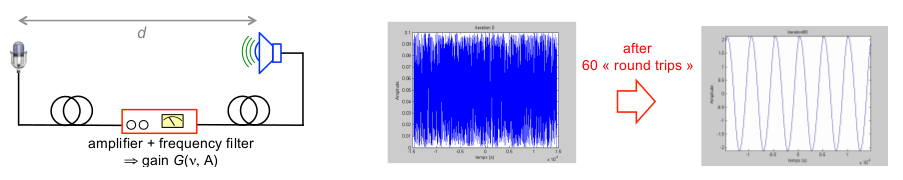
\includegraphics[scale=0.7]{ch7/image2.png}
	\captionof{table}{ }
	\end{wrapfigure}
	La seule chose pouvant varier dans cette expression est $\mu_r$ (il contient le cosinus de l'angle
	entre la direction d'entrée et de sortie). Comme cosinus est majoré par 1 et minoré par zéro, 
	on peut trouver un minimum d'énergie
	\begin{equation}
	{E_{\min }} = {\left( {\frac{{A - 1}}{{A + 1}}} \right)^2}E' \equiv \alpha \,E'
	\end{equation}
	La valeur $\alpha$ permet d'avoir un ordre de grandeur pour le ralentissement. L'hydrogène 
	fera ainsi un bon modérateur. Par contre si l'on veut ralentir l'$U^{238}$, il ne faut pas 
	être trop pressé.\\
	
	Il existe plusieurs relations entres les variables:
	\begin{itemize}
	\item[$\bullet$] $\mu_0=f(\mu_r)$ ; on utilise le rapport $v'/v$ avec le rapport des énergies (
	racine de l'inverse, où $\mu_r$ est la déflection angulaire dans le système absolu)
	\begin{equation}
	{\mu _o} = \frac{1}{v}\bar v.\bar \Omega ' = \frac{1}{v}\frac{{v'}}{{A + 1}}(\bar \Omega ' +
	 A{\bar \Omega _r}).\bar \Omega '  = \frac{1}{{A + 1}}\sqrt {\frac{{E'}}{E}} (A{\mu _r} + 1)
	 \Rightarrow  \to \;{\mu _o} = \frac{{A{\mu _r} + 1}}{{\sqrt {{A^2} + 2A{\mu _r} + 1} }}
	\end{equation}
	\item[$\bullet$] ${\mu _r} = f(E)$ ; inverse de l'expression ci-dessus (où $\mu_r$ est la 
	déflection angulaire dans le système du centre de masse)
	\begin{equation}
	{\mu _r} = \frac{{{{(A + 1)}^2}}}{{2A}}\frac{E}{{E'}} - \frac{{{A^2} + 1}}{{2A}}
	\end{equation}
	\item[$\bullet$] $\mu_0 = F(E)$ ; défini sur base des énergies
	\begin{equation}
	{\mu _o} = \frac{{A + 1}}{2}\sqrt {\frac{E}{{E'}}}  - \frac{{A - 1}}{2}\sqrt {\frac{{E'}}{E}} 
	\end{equation}
	\item[$\bullet$] ${\mu _r} = f({\mu _o})$
	\begin{equation}
	{\mu _r} = \frac{1}{A}(\mu _o^2 + {\mu _o}\sqrt {{A^2} - 1 + \mu _o^2}  - 1)
	\end{equation}
	\end{itemize}
	En laboratoire, on mesurera $\mu_0$ ($\mu_r$ est exprimé dans le référentiel du centre de 
	masse).
	
	\subsection{Loi de scattering}
	Il s'agit d'une fonction de densité de probabilité (\textit{pdf}) de l'angle de déflexion. 
	Celle-ci est habituellement donnée pour le système du centre de masse. Si le scattering 
	est isotrope (centre de masse)
	\begin{equation}
	p({\mu _r})d{\mu _r} = \frac{1}{2}d{\mu _r}
	\end{equation}
	où le facteur $1/2$ vient du $d\cos\theta$ dans l'élément d'angle solide. Ce qui nous intéresse, 
	c'est le mouvement observé au laboratoire. Grâce à la relation
	\begin{equation}
	p({\mu _r})d{\mu _r} = p({\mu _o})d{\mu _o}
	\end{equation}
	On peut écrire (en utilisant les relations entre variables décrites ci-dessus)
	\begin{equation}
	p({\mu _o}) = \frac{1}{{2A}}\left(   \frac{{{A^2} - 1 + 2\mu _o^2}}{{\sqrt {{A^2} - 1 +
	\mu _o^2} }} + 2{\mu _o}  \right) \quad\overset{A \gg 1}{\longrightarrow}\quad \frac{1}{2}
	\end{equation}
	Pour une masse de noyau tendant vers l'infini, on retrouve une densité de probabilité constante
	valant $1/2$. Ce résultat était attendu car si les masses tendent vers l'infini, il n'y a plus 
	de différence entre le mouvement absolu et relatif\footnote{Le "facteur de pondération" tend 
	vers $1/2$.}.\\
	
	Dans le cas où $A=1$
	\begin{equation}
	p({\mu _o}) = |{\mu _o}| + {\mu _o} = \left\{ {\begin{array}{*{20}{c}}
	{2{\mu _o}}&{si\,{\mu _o} > 0}\\
	0&{si\,{\mu _o} < 0}
	\end{array}} \right.
	\end{equation}
	Ceci ne concerne que le scattering vers l'\textit{avant}, il n'y a donc \textit{aucune} 
	rétro-diffusion ici\footnote{Limite du modèle ou réalité physique?}.\\
	
	On défini le \textbf{noyau de ralentissement} comme étant la fonction de densité de probabilité 
	de l'énergie d'un neutron ayant subit un scattering dans le cas isotropique. Sachant 
	que\footnote{Justif?} $K(E|E')dE = p({\mu _r})d{\mu _r}$, on trouve\\
	
	\cadre{\begin{equation}
	K(E|E') = \left\{ {\begin{array}{*{20}{c}}
	{\dfrac{1}{{(1 - \alpha )E'}}}&{if\,\alpha E' \le E \le E'}\\
	0&{else}
	\end{array}} \right.
	\end{equation}}\ \\
	
	On notera que le fait d'avoir un scattering isotrope dans le mouvement du centre de masse 
	n'implique pas que ce-dernier le soit également dans le mouvement absolu : quelque chose qui 
	va de l'avant peut être vu comme isotrope d'un point de vue relatif.\\
	
	De par la relation $K(E|E')dE = p({\mu _r})d{\mu _r}$, il est possible de calculer la \textit{
	perte d'énergie moyenne par collision élastique}\\
	
	\cadre{\begin{equation}
	 < E' - E >  = \int_{\alpha E'}^{E'}    (E' - E)K(E|E')dE = \frac{{(1 - \alpha )E'}}{2}
	\end{equation}}\ \\
	
	\begin{wrapfigure}[5]{r}{2.5cm}
	\vspace{-5mm}
	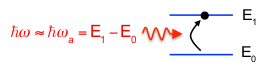
\includegraphics[scale=0.7]{ch7/image3.png}
	\captionof{table}{ }
	\end{wrapfigure}
	La valeur moyenne se trouve logiquement au centre de l'intervalle des énergies. Cette valeur 
	moyenne augmente avec $E'$ mais diminue avec $A$ car 
	\begin{equation}
	\frac{{(1 - \alpha )}}{2} = \frac{{2A}}{{{{(A + 1)}^2}}}
	\end{equation}

\newpage

	\subsection{Lethargie}
	\textit{Quoi de mieux qu'un lundi matin pour introduire une nouvelle variable énergie ?} En 
	effet, les dernières constatations poussent à introduire cette grandeur qui a \textit{augmente} 
	lorsque les neutrons \textit{ralentissent}\ \\
	
	\cadre{\begin{equation}
	u = \ln \frac{{{E_o}}}{E}
	\end{equation}
	Étant par définition positive, on en tire la valeur de l'état de référence $E_{ref}=E_0 : 
	u > 0 \forall E \to E_0 = 10\ $MeV.}\ \\
	
	Le but d'introduire cette variable est de pouvoir ré-écrire le noyau de ralentissement en 
	fonction de la lethargie $K(u|u')du = K(E|E')dE$. Pour se faire, il faut que\footnote{Pour 
	la suite, on défini $\ln\frac{1}{\alpha}\equiv q$.}
	\begin{equation}
	K(u|u')du = K(E|E')dE  = \frac{{{e^{ - (u - u')}}}}{{1 - \alpha }}du
	\end{equation}
	où $\alpha E' \le E \le E'\; \Rightarrow \;u' \le u \le u' + \ln \frac{1}{\alpha }$. Ceci 
	étant défini on peut faire le même raisonnement que pour l'énergie et calculer la 
	\textit{lethargie moyenne \textbf{gagnée} par collision élastique}
	\begin{equation}
	\xi  =  < u - u' >  = \int_{u'}^{u' + \ln \frac{1}{\alpha }}   (u - u')K(u|u')du = 1 -
	 \frac{\alpha }{{1 - \alpha }}\ln \frac{1}{\alpha }
	\end{equation}
	"\textit{Il s'agit d'une intégrale qui devrait vous être faisable en quatre jours}". On 
	remarque que ce résultat est \textit{indépendant} de $u'$ ! Le petit tour de passe-passe 
	opéré avec la lethargie est que, avec cette variable, le saut moyen qui va se faire n'est 
	plus qu'une caractéristique du noyau avec lequel il interagit. Après résolution
	\begin{equation}
	\xi  = 1 - \frac{{{{(A - 1)}^2}}}{{2A}}\ln \frac{{A + 1}}{{A - 1}}
	\end{equation}
	Avec un gain moyen en lethargie unitaire ($\xi=1$) pour l'hydrogène ($A=1$). Le point vraiment
	fondamental est que chaque collision, en moyenne, est une caractéristique de l'élément cible 
	indépendamment de l'énergie de départ et en plus la référence hydrogène correspond à un gain
	de 1, si c'est pas beau ça ! Le nombre moyen de collisions pour une augmentation de léthargie
	donnée est de
	\begin{equation}
	\Delta u = n\xi
	\end{equation}
	Ceci signifie que pour traverser une intervalle de lethargie $\Delta u$, il est nécessaire 
	de subir $n$ collisions pour traverser cet intervalle. \\
	
	\begin{wrapfigure}[8]{l}{9.5cm}
	\vspace{-8mm}
	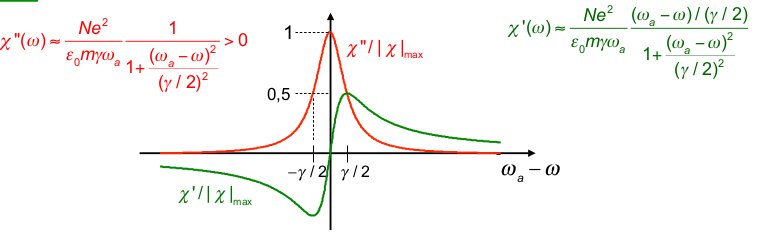
\includegraphics[scale=0.6]{ch7/image4.png}
	\captionof{table}{ }
	\end{wrapfigure}
	Ces grandeurs permettent de définir ce qu'est un modérateur efficace. Un bon modérateur présente
	un gain moyen en lethargie par collision le plus élevé que possible mais ce n'est pas 
	suffisant : il faut également avoir suffisamment de scattering sinon rien ne sera ralenti. 

	\newpage 
	On défini alors le \textbf{pouvoir de modération}
	\begin{equation}
	\text{Pouvoir de modération }: \quad \xi\Sigma_s
	\end{equation}
	Il faut que ce pouvoir de modération soit important, mais également l'absorption la plus faible
	que possible. On défini alors le \textbf{ratio de modération}
	\begin{equation}
	\text{Ratio de modération }: \quad \xi\Sigma_s/\Sigma_a		
	\end{equation}
	Le tableau en bas de la précédente page reprend les différents paramètres nous permettant de 
	choisir un \textit{bon} modérateur. 


	\subsection{Section efficace différentielle}
	Le lien entre la section efficace différentielle et la section totale de scattering est fait par
	le noyau de ralentissement\\
	
	\cadre{\begin{equation}
	{\Sigma _s}(\bar r,u' \to u) = {\Sigma _s}(\bar r,u')K(u|u')
	\end{equation}}\ \\
	
	On peut exprimer la section efficace différentielle en terme de lethargie et d'angles
	\begin{equation}
	{\Sigma _s}(\bar r,u',\bar \Omega ' \to u,\bar \Omega ) = {\Sigma _s}(\bar r,u')K(u|u')\frac{1}
	{{2\pi }}f({\mu _o})
	\end{equation}
	Comme précédemment, le cosinus de l'angle de déflection est déterminé par la cinématique des 
	collisions élastiques
	\begin{equation}
	{\mu _o} = \frac{{A + 1}}{2}\sqrt {\frac{E}{{E'}}}  - \frac{{A - 1}}{2}\sqrt {\frac{{E'}}{E}} 
	{\mu _o} = \frac{{A + 1}}{2}\sqrt {\frac{E}{{E'}}}  - \frac{{A - 1}}{2}\sqrt {\frac{{E'}}{E}} 
	\end{equation}
	On obtient une combili d'exponentielles contenant un delta en lethargie. Il en vient que
	\footnote{?}
	\begin{equation}
	f({\mu _o}) = \delta ({\mu _o} - {\mu _o}(u - u'))
	\end{equation}
	La facteur donnant la déflection angulaire est un delta de Dirac : un pic de variation correspond
	à \textbf{une} déflection angulaire: une variation donnée $\leftrightarrow$ une variation de 
	la lethargie.


\section{Équation de ralentissement}
	\subsection{Approximation $P_1$}
	L'objectif du ralentissement des neutrons est de déplacer le spectre d'énergie des neutrons dans 
	le domaine des collisions élastiques : la diffusion multi-groupe est nécessaire\footnote{On 
	cherche l'expression d'une loi de ralentissement permettant d'adapter le terme source.} et il faut
	prendre en compte les variations spatiales et d'énergie. \textit{Or}, nous n'avons pas de 
	variation spatiale du flux et donc pas de courant impliquant qu'il n'y a pas de diffusion ! Il 
	est dès lors possible de traiter la dépendance spatiale plus simplement.
	
	\subsubsection{Équation de Bolztmann stationnaire en lethargie}	
	Précédemment dans le cours de \textit{Physique des réacteurs nucléaires}, nous avions établi un
	lien entre $D$ et la section efficace (à une vitesse) :
	\begin{equation}
	D = \frac{1}{{3{\Sigma _{tr}}}}\quad\text{où}\quad {\Sigma _{tr}} = {\Sigma _t} -  < {\mu _o} >
	 {\Sigma _s}
	\end{equation}
	On lien avec la déflection angulaire était apparu. Ici, nous avons trouvé que
	\begin{equation}
	p({\mu _o}) = \frac{1}{{2A}}\left( \frac{{{A^2} - 1 + 2\mu _o^2}}{{\sqrt {{A^2} - 1 + \mu _o^2}
	 }} + 2{\mu _o}  \right)
	\end{equation}
	où $\langle\mu_0\rangle \neq 0$ (surtout si $A\approx 1$). Ceci nous donne l'idée de regarder 
	d'un peu plus près l'équation de Boltzmann, "\textit{ce qui n'est pas prendre un risque majeur}",
	écrite cette-fois en terme de lethargie\footnote{On change $v$ en $u$, les dimensions en sont un 
	peu affectées.}
	\begin{equation}
	\begin{array}{ll}
	div\bar J(\bar r,u,\bar \Omega )& \DS + {\Sigma _t}(\bar r,u)\varphi (\bar r,u,\bar \Omega )\\
	 &\DS - \int\limits_{4\pi }    \int_o^u    {\Sigma _s}(\bar r,u',\bar \Omega ' \to
	u,	\bar \Omega )\varphi (\bar r,u',\bar \Omega ')du'd\bar \Omega ' = S(\bar r,u,\bar \Omega )
	\end{array}	\end{equation}	
	Les fissions peuvent venir d'une éventuelle source extérieure donnée par
	\begin{equation}
	\begin{array}{ll}
	S(\bar r,u,\bar \Omega )&\DS = \frac{1}{{4\pi }}\int_{}^{}    {\Sigma _{in}}(\bar r,u' \to u)
	\varphi (\bar r,u')du'\\
	&\DS+ \frac{1}{{4\pi }}\chi (u)\int\limits_{4\pi }   \int_o^u   \nu {\Sigma _f}(\bar r,u')\varphi
	(\bar r,u',\bar \Omega ')du'd\bar \Omega ' + Q(\bar r,u,\bar \Omega )
	\end{array}
	\end{equation}		
	\textit{On va reprendre une vieille connaissance} : l'hypothèse d'anisotropie faible qui nous 
	avait donné le développement du flux suivant
	\begin{equation}
	\varphi (\bar r,u,\bar \Omega ) = \frac{1}{{4\pi }}(\varphi (\bar r,u) + 3\bar \Omega .\bar 
	J(\bar r,u))
	\end{equation}
	En absence de dépendances énergétiques, on va substituer ces équations dans l'équation de 
	Boltzmann et prendre le moment à l'ordre zéro : flux intégrer, plus de dépendance en 
	$\bar{\Omega}$ dans la divergence et la section différentielle ne va plus qu'être fonction 
	de la position et la lethargie :\\
	
	\cadre{
	\begin{equation}
	\int\dots \text{d}\bar\Omega \quad\Rightarrow\quad 
	div\bar J(\bar r,u) + {\Sigma _t}(\bar r,u)\varphi (\bar r,u) - \int_o^u  {\Sigma _s}(\bar r,u'
	\to u)\varphi (\bar r,u')du' = S(\bar r,u)
	\end{equation}}\ \\
	
	Prenons maintenant le moment d'ordre 1. Par isotropie, le membre de droite s'annule lors de 
	l'intégration\\
	
	\cadre{\begin{equation}
	\int\dots \bar\Omega\text{d}\bar\Omega \quad\Rightarrow\quad 	
	\frac{1}{3}\bar \nabla \varphi (\bar r,u) + {\Sigma _t}(\bar r,u)\bar J(\bar r,u) - \int_o^u  
	{\Sigma _{s1}}(\bar r,u' \to u)\bar J(\bar r,u')du' = 0
	\end{equation}
	où ${\Sigma _{s1}}(\bar r,u' \to u) = \int_{\bar \Omega }^{}    {\Sigma _s}(\bar r,u',\bar \Omega
	 ' \to u,\bar \Omega )\bar \Omega '.\bar \Omega d\bar \Omega $.	
	}\ \\
	
	Regardons plus en détail l'expression de $\Sigma_{s1}$. Bien qu'étant le résultat d'une petite
	manipulation, mais il s'agit surtout d'un $\Sigma_s$ avec une dépendance en lethargie. Dans le 
	cas mono-énergétique, nous avons une expression dépendant de la moyenne de la déflection 
	angulaire\footnote{${\Sigma _{tr}} = {\Sigma _t} -  < {\mu _o} > {\Sigma _s}$}. Ici, nous 
	avons $\Sigma_{s,total}$ multiplié par un noyau de scattering et la déflection angulaire, le tout
	multiplié par $\bar{\Omega'}\bar\Omega$. Il s'agit bien de lavaleur moyenne de la déflection 
	angulaire car la distrubtion de cette déflexion est multipliée par cette même déflection : c'est
	la définition de la moyenne statistique. \\
	
	Dans le cas où plusieurs isotopes sont présent, on travaille avec une "mixture" :${\Sigma _s}
	(\bar r,u' \to u) = \sum\limits_i  {\Sigma _{si}}(\bar r,u'){K_i}(u|u')$. On en tire
	\begin{equation}
	{\Sigma _{s1}}(\bar r,u' \to u) = \sum\limits_i  {\Sigma _{si}}(\bar r,u'){K_i}(u|u'){\mu 
	 _{oi}}(u - u')
	\end{equation}
	
	
	\subsection{Densité de ralentissement}	
	Il s'agit du nombre de neutrons (par unité de volume et de temps) ralenti au dessus\footnote{On 
	se rappelle qu'un ralentissement des neutrons cause une augmentation de la léthargie.} d'une 
	lethargie $u$ en un point et direction donnée (version angulaire)\\
	
	\cadre{
	\begin{equation}
	q(\bar r,u,\bar \Omega ) = \int_o^u   \int_{\bar \Omega '}^{}    \left( \int_u^
	\infty     {\Sigma _s}(\bar r,u',\bar \Omega ' \to u,\bar \Omega )du    \right)\varphi
	(\bar r,u',\bar \Omega ')du'd\bar \Omega '
	\end{equation}}\ \\
	
	Il existe aussi une version débarrassée de la partie angulaire que l'on nomme \textbf{densité 
	de ralentissement} (version intégrée donc)\ \\
	
	\cadre{\begin{equation}
	\begin{array}{ll}
	q(\bar r,u) &\DS= \int_o^u   \left(   \int_u^\infty    {\Sigma _s}(\bar r,u' \to u)du
	\right)\varphi (\bar r,u')du'\vspace{2mm}\\
	&=\DS  \int_o^u   \left(  \int_u^\infty     K(u|u')du  \right){\Sigma _s}(\bar r,u')\varphi 
	(\bar r,u')du'
	\end{array}
	\end{equation}}\ \\
	
	On retrouve tout d'abord un terme $\Sigma_s\varphi$ que l'on intègre de 0 à $u$ pour comptabiliser
	les neutrons qui ont une léthargie inférieure à $u$ et qui vont passer au dessus de ce seuil. 
	Ensuite, il faut intégrer sur $du'$ de $u$ à $\infty$ le noyau de ralentissement qui va faire 
	passer les léthargie $u''$ à $u$. De cette façon, on a repris tous les neutrons qui sont ralentis 
	à une léthargie au dessus d'une léthargie donnée. Ce raisonnement est aussi applicable au cas
	angulaire.\\
	
	Il est également possible (à condition d'aimer les intégrales) de définir une \textit{densité de
	courant de ralentissement}
	\begin{equation}
	\begin{array}{ll}
	{\bar q_1}(\bar r,u) &\DS= \int_{\bar \Omega }^{}    \int_o^u    \int_{\bar \Omega '}^{}    \left( 
	\int_u^\infty    {\Sigma _s}(\bar r,u',\bar \Omega ' \to u,\bar \Omega )du  \right)\bar \Omega
	\varphi (\bar r,u',\bar \Omega ')du'd\bar \Omega 'd\bar \Omega\vspace{2mm}\\
	 &\DS = \int_o^u    \left( \int_u^\infty     {\Sigma _{s1}}(\bar r,u' \to u)du  \right)\bar 
	 J(\bar r,u')du'\vspace{2mm}\\
	&\DS= \int_o^u    \left(   \int_u^\infty     K(u|u')du   \right){\Sigma _{s1}}(\bar r,u')\bar
	J(\bar r,u')du'
	\end{array}
	\end{equation}\ \\
	
	Il peut être intéressant d'avoir l'expression de la \textbf{variation de densité de 
	ralentissement}\footnote{\textbf{Interprétation physique manquante!!}}
	\begin{equation}
	\frac{{\partial q(\bar r,u)}}{{\partial u}} = {\Sigma _s}(\bar r,u)\varphi (\bar r,u) - \int_o^u 
	 {\Sigma _s}(\bar r,u' \to u)\varphi (\bar r,u')du'
	\end{equation}
	En prenant le moment au premier ordre, le $\Sigma$ non élastique qui est dans le domaine de
	résonance tend directement vers l'absorption
	\begin{equation}
	div\bar J(\bar r,u) + {\Sigma _{ne}}(\bar r,u)\varphi (\bar r,u) + \frac{{\partial q(\bar r,u)}}
	{{\partial u}} = S(\bar r,u)
	\end{equation}
	où ${\Sigma _{ne}}(\bar r,u) = {\Sigma _t}(\bar r,u) - {\Sigma _s}(\bar r,u) = {\Sigma _a}(\bar
	 r,u) + {\Sigma _{in}}(\bar r,u)\longleftrightarrow{\Sigma _a}(\bar r,u)$.\\
	 
	 Nous avons également la \textbf{variation de la densité de courant de ralentissement}
	 \begin{equation}
	 \frac{{\partial {{\bar q}_1}(\bar r,u)}}{{\partial u}} = {\Sigma _{s1}}(\bar r,u)\bar J(\bar r,u)
	  - \int_o^u  {\Sigma _{s1}}(\bar r,u' \to u)\bar J(\bar r,u')du'
	 \end{equation}
	 En prenant le moment d'ordre 1 : 
	 \begin{equation}
	 \frac{1}{3}\bar \nabla \varphi (\bar r,u) + {\Sigma _{tr}}(\bar r,u)\bar J(\bar
	  r,u) + \frac{{\partial {{\bar q}_1}(\bar r,u)}}{{\partial u}} = 0
	 \end{equation}
	 où ${\Sigma _{tr}}(\bar r,u) = {\Sigma _t}(\bar r,u) - {\Sigma _{s1}}(\bar r,u) = {\Sigma _t}
	 (\bar r,u) - \sum\limits_i     < {\mu _{oi}} > {\Sigma _{si}}(\bar r,u)$.
	 
	 \subsubsection{Équations de ralentissement : résumé}
	 En dehors des domaines thermiques et rapides, nous avons quatre équations\footnote{Peut-être
	 revoir les noms, je suis plus certain.}\\
	 
	 \cadre{\begin{enumerate}
	 \item Moment d'ordre 0 de la variation de la densité de ralentissement
	 \begin{equation}
	 div\bar J(\bar r,u) + {\Sigma _{ne}}(\bar r,u)\varphi (\bar r,u) + \frac{{\partial q(\bar r,u)}}
	 {{\partial u}} = S(\bar r,u)
	 \end{equation}
	 \item Densité de ralentissement
	 \begin{equation}
	 q(\bar r,u) = \int_o^u    \left( \int_u^\infty     K(u|u')du  \right)	 {\Sigma _s}(\bar r,u')
	 \varphi (\bar r,u')du'
	 \end{equation}
	 \item Moment d'ordre 1 de la variation de la densité de ralentissement
	 \begin{equation}
	 \frac{1}{3}\bar \nabla \varphi (\bar r,u) + {\Sigma _{tr}}(\bar r,u)\bar J(\bar r,u) +
	  \frac{{\partial {{\bar q}_1}(\bar r,u)}}{{\partial u}} = 0
	 \end{equation}
	 \item Densité de courant de ralentissement
	 \begin{equation}
	{\bar q_1}(\bar r,u) = \int_o^u   \left(   \int_u^\infty    K(u|u')du \right){\Sigma
	  _{s1}}(\bar r,u')\bar J(\bar r,u')du'
	 \end{equation}
	 \end{enumerate}}
	 
	 
	 
	\subsection{Matériau homogène infini}
	Le fait de travailler en milieu infini permet de se débarrasser de la dépendance spatiale (la 
	divergence étant nulle en milieu infini)
	\begin{equation}
	{\Sigma _t}(u)\varphi (u) - \int_o^u    {\Sigma _s}(u' \to u)\varphi (u')du' = S(u)
	\end{equation}
	A partir de cette expression, définissions le premier terme comme la \textbf{densité de collision}
	\footnote{Ne pas confondre la \textit{densité de collision} avec les \textit{pdf}.} 
	\begin{equation}
	F(u) = {\Sigma _t}(u)\varphi (u)
	\end{equation}
	La probabilité de scattering pour un isotope $i$ est logiquement obtenue en faisant le rapport 
	entre la section efficace de scattering sur l'élément $i$ sur la section efficace totale
	\begin{equation}
	{c_i}(u) = \frac{{{\Sigma _{si}}(u)}}{{{\Sigma _t}(u)}}
	\end{equation}
	Si le scattering est isotropique, on trouve l'équation de ralentissement des neutrons en 
	milieu infini\ \\
	
	\cadre{\begin{equation}
	F(u) - \sum\limits_i  \frac{1}{{1 - {\alpha _i}}}\int_{\max (0,u - {q_i})}^u   {e^{u' - u}}{c_i}
	(u')F(u')du' = S(u)
	\label{eq:Ch7.InfMed}
	\end{equation}
	où ${q_i} = \ln \frac{1}{{{\alpha _i}}}$. Notons que $F(u)$ et $c_i(u)$ sont plus "doux" que 
	$\Sigma_t(u)$ et $\varphi(u)$.}\ \\
	
	De façon similaire, on peut écrire à partir du moment d'ordre zéro la \textbf{densité de 
	ralentissement}\ \\
	
	\cadre{\begin{equation}
	\frac{{dq(u)}}{{du}} = S(u) - {\Sigma _a}(u)\varphi (u)
	\end{equation}}\ \\
	
	S'il n 'y a pas d'absorption, la densité de ralentissement est donnée par intégration directe 
	de la source. Pour une source $S(u) = \chi (u){S_o}$, on trouve 
	\begin{equation}
	q(u) = \int_o^u  \chi (u)du\,{S_o}
	\end{equation}
	S'il n'y a pas d'absorption, la variation de la densité représente ce qui n'a pas été 
	absorbé. On définit alors la \textbf{probabilité anti-trappe}\footnote{ou \textit{probabilité 
	d'échapper à la résonance si $E$ est la borne supérieure de l'énergie thermique.}}
	\begin{equation}
	q(E)/S_0
	\end{equation}
	Il s'agit de la probabilité de ne pas se faire absorbé entre $E_{source}$ et $E$ (la borne 
	supérieure de l'énergie thermique).
	
	
	
\section{Ralentissement dans l'hydrogène}
	\subsection{Hypothèses}
	Nous allons faire l'hypothèse d'un milieu infini où l'absorption dans l'hydrogène est 
	négligeable. La ralentissement considéré se situe dans le domaine de résonnance et ceux-ci se
	feront de façon élastiques avec les noyaux légers : pas assez d'énergie pour avoir du 
	scattering inélastique et le ralentissement par noyaux lourds est négligeable. 
	En bref, les noyaux lourds s'occupent de l'absorption et l'hydrogène du ralentissement.
	
	
	\subsection{Forme de flux}
	Rappelons que pour l'hydrogène, $\alpha_i=0$. L'équation de ralentissement \eqref{eq:Ch7.InfMed}
	s'écrit alors	
	\begin{equation}
	F(u) - \int_o^u    {e^{u' - u}}c(u')F(u')du' = S(u)
	\end{equation}
	
	Comme\footnote{TT : il faut vérifier si c'est correct}
	\begin{equation}
	\frac{dF(u)}{du} - c(u)F(u) +\overbrace{\int_0^u e^{u’-u} c(u’)F(u’)du’}^{\equiv F(u)-S(u)} =
	\frac{dS}{du}
	\end{equation}
	Et donc
	\begin{equation}
	\frac{{dF(u)}}{{du}} + (1 - c(u))F(u) = \frac{{dS(u)}}{{du}} + S(u)
	\end{equation}		
	Il s'agit d'une équation du premier ordre. On trouve comme SGEH 
	\begin{equation}
	e^{\int^u (1-c(u’)du’}
	\end{equation}
	On va procéder à la variation des constantes pour la SPEnH en cherchant une solution de la 
	forme $A(u) e^{\int^u (1-c(u’)du’}$. En la substituant
	\begin{equation}
	A(u) e^{\DS\int^u (1-c(u^{’})du^{’}}  = \int^u\left[ S(u’)+\dfrac{dS(u’)}{du’}\right]
	e^{\DS-\int_{u’}^u (1-c(u"))du"}du’
	\end{equation}
	En simplifiant, on peut en tirer $F(u)$
	\begin{equation}
	F(u) = \left[ S(u’) e^{-\int_{u’}^u (1-c(u"))du"}\right]_0^u + \int_0^u
	\left[S(u’)-S(u’)(1-c(u’))\right]e^{\dots} du’
	\end{equation}
	Soit encore (je sais pas comment on a justifier ces équations\dots\\ \\
	
	\cadre{\begin{equation}
	F(u) = S(u) + \int_o^u  {e^{ - \int_{u'}^u    (1 - c(u))du}}c(u')S(u')du'
	\end{equation}}\ \\
	
	Si la source est mono-cinétique $S(u) = {S_o}\delta (u - {u_o})$ on trouve\\
	
	\cadre{
	\begin{equation}
	F(u) = {e^{ - \int_{{u_o}}^u   \frac{{{\Sigma _a}(u')}}{{{\Sigma _t}(u')}}du'}}\frac{{{\Sigma _s}
	({u_o})}}{{{\Sigma _t}({u_o})}}{S_o}
	\end{equation}}\ \\
	
	Il s'agit de l'expression dans un milieu infini pour une source monoénergétique où seul 
	l'hydrogène ralenti les neutrons. La solution pour une source générale s'obtient par combinaisons 
	de cette solutions.\\
	
	Pour traiter le cas sans absorption, il est plus commode de d'abord repasser en variable 
	énergie. Pour se faire, il faut que $\varphi(E)dE=\varphi(u)du$. Comme la léthargie est donnée 
	par le logarithme de $E_0/E$, on trouve un facteur $1/E$ lors du calcul de $du$ :
	\begin{equation}
	\varphi (u) = \frac{{{S_o}}}{{{\Sigma _t}(u)}}\qquad\Rightarrow\qquad
	\varphi (E) = \frac{{{S_o}}}{{{\Sigma _t}(E)E}}
	\end{equation}
	
	Attardons nous quelque-peu sur le cas avec absorption. On considère que, en dehors des 
	résonance pour $\varphi(E)$, on retrouve le même comportement que lorsque l'on avait 
	négligé l'absorption ($\Sigma_a$ négligeable). Après chaque résonance le flux doit être réduit :
	le facteur de réduction est donné par
	\begin{equation}
	{e^{\DS - \int_{res}^{}    \frac{{{\Sigma _a}(u')}}{{{\Sigma _t}(u')}}du'}}
	\end{equation}
	Sur tout le domaine, et donc l'ensemble des résonance, il faut sommer
	\begin{equation}
	{e^{\DS - \int_{{u_o}}^u  \frac{{{\Sigma _a}(u')}}{{{\Sigma _t}(u')}}du'}} = {e^{\DS - \sum
	\limits_{res	 < u}   \,\int\limits_{res}   \frac{{{\Sigma _a}(u')}}{{{\Sigma _t}(u')}}du'}}
	\end{equation}
	Le flux se réduira donc systématiquement de ce facteur (expression importante).

	\subsection{Forme de la densité de ralentissement}
	Repartons de la définition quelque peu modifiée\footnote{Interprétation physique donnée plus
	haut.}
	\begin{equation}
	q(u) = \int_o^u   \left( \int_u^\infty    {e^{u' - u}}du\right)c(u')F(u')du' 
	= \int_o^u  {e^{u' - u}}c(u')F(u')du' = F(u) - S(u)
	\end{equation}
	Nous avons vu que, pour une source à une vitesse ($u_0$), une vitesse de densité de ralentissement 
	correspondait à un type de collision\footnote{Phrase à éclaircir}. Si $u>u_0$
	\begin{equation}
	q(u) = {e^{ - \int_{{u_o}}^u    (1 - c(u'))du'}}c({u_o}){S_o}
	\end{equation}
	Si on refait le raisonnement tenu en milieu infini pour la probabilité anti-trappe, celle-ci est 
	donnée par une exponentielle décroissante qui sera potentiellement sommée sur toute les 
	résonance que l'on trouve dans le domaine
	\begin{equation}
	p(u) = \frac{{q(u)}}{{q({u_o})}} = \exp \left( { - \int_{{u_o}}^u    \frac{{{\Sigma _a}(u')}
	}{{{\Sigma _t}(u')}}du'} \right)
	\end{equation}

	
\section{Autres modérateurs}
	Comme je sais que tu es assez fainéant, voici l'expression obtenue en milieu infini homogène
	\begin{equation}
	F(u) - \sum\limits_i  \frac{1}{{1 - {\alpha _i}}}\int_{\max (0,u - {q_i})}^u  {e^{u' - u}}{c_i}
	(u')F(u')du' = S(u)
	\end{equation}
	
	\subsection{Fonction de Placzek}
	L'idée est d'introduire une fonction $P(u)$ qui remplace la densité de collisions $F(u)$ si et
	seulement si
	\begin{itemize}
	\item[$\bullet$] Un seul matériau
	\item[$\bullet$] Pas d'absorption
	\item[$\bullet$] Source mono-cinétique
	\end{itemize}	
	On écrit alors\\
	
	\cadre{\begin{equation}
	P(u) - \int_o^\infty     K(u - u')P(u')du' = \delta (u)
	\end{equation}
	où $K(u) = \frac{1}{{1 - \alpha }}{e^{ - u}}H(u)H(q - u)$.}\ \\
	
	
	Mais oui, tu l'as remarqué ! Une magnifique convolution est présente, on va prendre la transformée 
	de Laplace
	\begin{equation}
	\bar K(p) = \frac{{1 - {\alpha ^{p + 1}}}}{{(1 - \alpha )(1 + p)}}\quad\Rightarrow\quad
	\bar P(p) - \bar K(p)\bar P(p) = 1
	\end{equation}	 
	
	\textit{Notes de cours}\footnote{Heuu\dots ?}
	\begin{equation}
	\bar K (p) = \int_0^q \frac{e^{-u}}{1-\alpha}e^{-p}du = \frac{1}{1-\alpha} \frac{1}{1+p}\left(1-\underbrace{e^{-(1+p)q}}_{\alpha^{(p+1)}}\right)
	\end{equation}
	La transformée de la fonction de Paczek peut s'écrire comme le noyau + une fois la convolution 
	+ deux fois la convolutions +\dots ce qui nous sera utile pour repasser simplement en léthargie :
	\begin{equation}
	\bar P(p) = \frac{1}{{1 - \bar K(p)}} = 1 + \bar K(p) + {\bar K^2}(p) + \dots
	\end{equation}
	
	Ceci étant fait, on peut s'intéresser aux solutions de notre fameuse équation
	\begin{equation}
	P(u) = \delta (u) + \int_{\max (0,u - q)}^u   \frac{{{e^{u' - u}}}}{{1 - \alpha }}P(u')du'
	\end{equation}
	Pour la résoudre, il faut décomposer le problèmes en plusieurs intervalles
	\begin{itemize}
	\item[$\bullet$] A l'origine, les bornes de l'intégrale tendent toutes deux vers zéro et la 
	contribution de celle-ci est nule : $P(u) = \delta (u)$.
	\item[$\bullet$] Premier intervalle : $0<u<q$. L'équation se ramène à
	\begin{equation}
	P(u) = \int_0^u \frac{e^{u’-u}}{1-\alpha}du’
	\end{equation}
	Soit encore
	\begin{equation}
	\frac{dP(u)}{du} = \frac{P(u)}{1-\alpha}-P(u) = \frac{\alpha}{1-\alpha} P(u)
	\end{equation}
	On en tire
	\begin{equation}
	P(u) = \frac{{\exp (\frac{{\alpha u}}{{1 - \alpha }})}}{{1 - \alpha }}
	\end{equation}
	\item[$\bullet$] \textit{Discontinuité}. A l'origine on retrouve un pic de Dirac, valable 
	uniquement pour une léthargie positive. Comment alors arriver à la solution générale 
	$\propto e^{\frac{\alpha}{1-\alpha}u}$ à celle ci-dessus?  On peut dire que
	\begin{equation}
	P(u) = P(0+) e^{\frac{\alpha}{1-\alpha}u} 
	\end{equation}
	Si on regarde 
	\begin{equation}
	P(u) = \int_0^u \frac{e^{u’-u}}{1-\alpha}du’ 
	\end{equation}
	Le tout tendant vers zéro, on retrouve juste une contribution pour $u'$ centrée à l'origine, c'est
	$\delta(u)$. Il y a donc une discontinuité\footnote{Pas clair\dots} :
	\begin{equation}
	q : - \frac{\alpha }{{1 - \alpha }}
	\end{equation}
	\item Second intervalle : $q<u<2q$. L'équation se ramène à
	\begin{equation}
	\int_{u-q}^u \frac{e^{u’-u}}{1-\alpha}P(u’)du’\qquad\Leftrightarrow\qquad
	\frac{dP(u)}{du} = \frac{P(u)}{1-\alpha} -\frac{e^{-q}P(u-q)}{1-\alpha}-P(u)
	\end{equation}
	De façon plus propre
	\begin{equation}
	P(u) = \frac{{\exp ({\textstyle{{\alpha u} \over {1 - \alpha }}})}}{{1 - \alpha }}(1 - {\alpha
	 ^{\frac{1}{{1 - \alpha }}}} - \frac{\alpha }{{1 - \alpha }}(u - q))
	\end{equation}
	On voit l'apparition d'un terme supplémentaire : pour "nourrir" cette ED, on ne peut que prendre 	
	la solution sur le premier intervalle
	\end{itemize}\ 
	
	La résolution du problème se fait donc intervalle par intervalle ; on part d'un pic de Dirac, 
	on arrive à une discontinuité $(q^+)$ car plus de pic de Dirac et on continue.\\
	
	\begin{wrapfigure}[11]{r}{3cm}
	\vspace{-5mm}
	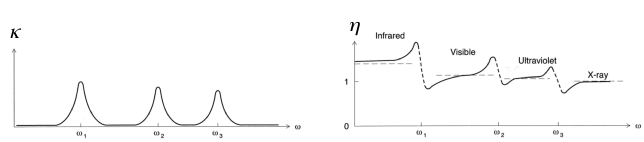
\includegraphics[scale=0.4]{ch7/image5.png}
	\captionof{figure}{ }
	\end{wrapfigure}
	La résolution se fait donc intervalle par intervalle. Par les théorèmes taubériens, il est 
	possible de déterminer le comportement pour un temps infini
	\begin{equation}
	{P_\infty } = \mathop {\lim }\limits_{p \to 0} p\bar P(p)\; = \mathop {\lim }\limits_{p \to 0}
	 \frac{p}{{1 - \bar K(p)}} \to \frac{1}{\xi }
	\end{equation}
	Il y a donc des oscillations au voisinage de l'origine nommée les \textit{oscillations de Placzek}
	puis une convergence vers une valeur constante\footnote{Section  revoir++}.




\section{Dépendance spatiale}
	\subsection{Théorie de l'age de Fermi}
	Nous allons utiliser les équations à un groupe ($P_1$) en utilisant l'\textit{approximation 
	d'âge}
	\begin{equation}
	q(\bar r,u) = \bar \xi (u){\Sigma _s}(u)\varphi (\bar r,u)
	\end{equation}
	où $\bar\xi$ est le décrément logarithmique moyen dans le cas où plusieurs isotopes sont présent. 
	Autre hypothèse : nous négligeons $\frac{{\partial {{\bar q}_1}(\bar r,u)}}{{\partial u}}$ dans
	l'équation du courant qui s'écrit alors
	\begin{equation}
	\bar J(\bar r,u) =  - \frac{1}{{3{\Sigma _{tr}}(\bar r,u)}}\bar \nabla \varphi (\bar r,u) =  -
	 D(\bar r,u)\bar \nabla \varphi (\bar r,u)
	\end{equation}
	Comme nous avons également (moment d'ordre zéro)
	\begin{equation}
	 - div(D(\bar r,u)\bar \nabla \varphi (\bar r,u)) + {\Sigma _a}(\bar r,u)\varphi (\bar r,u) +
	  \frac{{\partial q(\bar r,u)}}{{\partial u}} = S(\bar r,u)
	\end{equation}		
	Il est possible d'obtenir un lien direct entre la densité de ralentissement et le flux en 
	substituant cette expression dans celle du courant. On obtient alors, pour toute zone homogène et 
	pour une léthargie supérieure à celles des sources considérées ici :\\
	
	\cadre{\begin{equation}
	\frac{{D(u)}}{{\bar \xi (u){\Sigma _s}(u)}}\Delta q(\bar r,u) - \frac{{{\Sigma _a}(\bar r,u)}}
	{{\bar \xi (u){\Sigma _s}(u)}}q(\bar r,u) - \frac{{\partial q(\bar r,u)}}{{\partial u}} = 0
	\end{equation}
	où, pour rappel, $\Sigma_a/d$ est la longueur de diffusion.}\ \\
	
	Fort inspiré de cette dernière relation, définissons l'\textbf{age des neutrons}\footnote{\danger\ 
	Unités exprimées en [$cm^2$] !} \ \\
	
	\cadre{\begin{equation}
	\tau (u) \equiv \int_o^u  \frac{{D(u')}}{{\bar \xi (u'){\Sigma _s}(u')}}du'
	\end{equation}}\ \\
	
	On peut alors obtenir l'\textbf{équation de Fermi}
	\begin{equation}
	\Delta q(\bar r,\tau ) - \frac{1}{{{L^2}(\tau )}}q(\bar r,\tau ) - \frac{{\partial q(\bar r,\tau
	 )}}{{\partial \tau }} = 0
	\end{equation}
	Soit $q(\bar r,\tau ) = p(\tau )\tilde q(\bar r,\tau )$ avec la probabilité anti-trappe donnée 
	par
	\begin{equation}
	p(\tau ) = {e^{\DS - \int_o^{u(\tau )}    \frac{{{\Sigma _a}(u')}}{{\bar \xi {\Sigma _s}(u')}}
	du'}} = {e^{\DS - \int_o^\tau     \frac{1}{{{L^2}(\tau ')}}d\tau '}}
	\end{equation}
	où $p$ a été ré-exprimée en fonction de cette variable âge. On retrouve le facteur $1/L^2$ 
	(longueur de diffusion). La subtilité de cette  transformation avec cette densité de 
	ralentissement purement migratoire (diffusive) est que lorsque l'on dérive la densité de 
	ralentissement par rapport à l'age (équation de Fermi) on fait apparaître ce facteur 
	$1/L^2$ qui se simplifie avec le second terme de cette même équation. Comme le laplacien ne 
	porte pas sur la probabilité anti-trappe mais seulement sur les coordonnées spatiales, on 
	trouve\\
	
	\cadre{\begin{equation}
	\Delta \tilde q(\bar r,\tau ) = \frac{{\partial \tilde q(\bar r,\tau )}}{{\partial \tau }}
	\end{equation}}\ \\
	
	Fermi nous ramène aussi à une équation de diffusion ressemblant à une équation dépendante du
	temps. 	C'est d'ailleurs une forme tout à fait semblable à celle que l'on aurait obtenue pour 
	un problème dépendant du temps, si ce n'est que la variable "temporelle", l'age, est en 
	réalité une variable énergie ! C'est comme si le temps est remplacé par un accroissement de 
	type léthargie mais un peu plus compliquée.
	
	\subsubsection{Relation léthargie - temps}
	Supposons que l'on soit en présence de noyaux suffisamment lourds : à chaque scattering élastique
	avec des noyaux, la léthargie n'augmentera que peu. Si cette quantité est relativement petite, 
	assez intuitivement, on n'aura que peu de variation par rapport à un chemin moyen que prendrait 
	un neutron et fur et à mesure qu'il subit des collisions : on peut se dire que \textit{tous les
	neutrons ralentissent comme un seul homme, ou plutôt comme un seul neutron}.\\
	
	Comme tous les neutrons ont un ralentissement semblable (ou avec une faible variabilité), la 
	léthargie sera une \textbf{fonction du temps de ralentissement} !\\
	
	Considérons l'équation de diffusion (dont le membre de droite est nul, car pas de matière 
	fissile) au temps $t$ (pour un neutron émis à $t=0$ avec $u=0$) :
	\begin{equation}
	\frac{1}{v}\frac{{\partial \varphi (\bar r,t)}}{{\partial t}} - div(D(\bar r,t)\bar \nabla \varphi
	(\bar r,t)) + {\Sigma _a}(\bar r,t)\varphi (\bar r,t) = 0
	\end{equation}
	Intéressons-nous à la variation de léthargie par rapport au temps 
	\begin{equation}
	du = \bar \xi {\Sigma _s}vdt
	\end{equation}
	Si $\Sigma_s$ est la probabilité par unité de longueur d'avoir un scattering élastique, la 
	multiplication de ce-dernier par la vitesse $v$	donne la probabilité par unité de temps qu'un 
	scattering élastique se produise. Le nombre de scattering élastique que l'on va rencontrer dans 
	un intervalle de temps $dt$ est alors donné par $\Sigma_svdt$. La variation de léthargie que l'on
	va avoir s'ils adoptent tous le même comportement moyen est donnée en multipliant ce triple 
	produit par le décrément logarithmique $\bar \xi$, soit le gain de léthargie par collision.\\
	
	Si l'on effectue ce changement de variable dans l'équation juste au dessus, on retombe sur 
	l'équation de Fermi ! Nous avons ainsi pu écrire un lien univoque entre la variation du temps 
	et de la léthargie, mais ceci n'est hélas vrai que pour des atomes suffisamment lourd, comme 
	c'est le cas pour le graphite en pratique\footnote{Le slide 26 donne des exemples de noyaux 
	de ralentissement et la fin du chapitre n'est pas à connaître ! Retenons cependant que l'age 
	est directement lié à la longueur de diffusion durant la modération, ce qui donne une autre 
	interprétation physique de cette grandeur.}.